\section{Define the Problem of Mapping the Software Applications}\label{sec_problem}
The software applications $A$ are partitioned on the execution platform $\langle N,B\rangle$ by fulfilling the user-defined software applications requirements such as applications reliability $\ssp{RL}$, end-to-end timing requirements of chains $\sss{EE}$ and software applications criticality $\ssp{cl}$, and by meeting design constrains such as placement restrictions committed by the designer. The partitioning  is conducted by mapping the respective software-component replicas (or software components in short) of applications effectively on the computing units $M'$ and the communication between software components on the network bus. The partitioning should result in reduced total power-consumption of the applications $Power(\textbf{x})$, which is achieved by selecting lower-power computing units $N'\subseteq N$, where $\textbf{x}$ is a possible partitioning matrix (or partition in short) with \ttxkij representing the mapping of the software component \ttsss{q}[k][i,j] to the compuing node $n_h$, where $h=\xkij$.  Note: under this partition, the reliability of applications $Reliability_{A_k}(\textbf{x})$, the timing of chains $Delay_{\sss{\Gamma}}(\textbf{x})$ should satify the respective requirements. 

%The solution to the allocation problem is represented by a vector-matrix $\x=\{\xsp{A_k}:k=1,...,N_a\}$ as shown in Equation (\ref{eqn_solution}), where \ttxsp{k} is a matrix of size $n_C\times K$, and \ttssx{x}{k}{ij}$=h\in \{1,…,n_N\}$ denotes the mapping of the  software-component replica \ttssx{q}{k}{i,j} to the computinG node $n_h$.
%\begin{equation}
%\label{eqn_solution}
%\bspx{k}=
%\begin{bmatrix} 
%\ssx{k}{11} & \ssx{k}{12} & \dots & \ssx{k}{1K}\\
%\ssx{k}{21} & \ssx{k}{22} & \dots & \ssx{k}{2K}\\
%\vdots & \vdots & \ddots & \vdots\\
%\ssx{k}{N_c1} & \ssx{k}{N_c2} & \cdots & \ssx{k}{N_cK}
%\end{bmatrix}
%\end{equation}

The power consumption of applications as well as the delay of chains depend on the tasks graphs $\bigcup\sss{g}[k][\tau]$, as well as the mapping of the tasks nodes to computing units and the links to the network bus. In this case, the tasks graphs has be constructed from the partition \ttx. However, if the tasks graphs are apriori to the software partitioning problem,  which can be the case if no runnables from different components map to a single task, only the tasks nodes and the links has to be updated with the mapping information.

\subsection{Task Graph Formulation}
The task graph formulation implies the generation of a task graph, with the cost over the tasks nodes and the links updated for the partition \ttx. The tasks nodes are updated with the timing information and the mapping to computing units, likewise, the links with the mapping to the network bus. The formulation has two steps: i) for a mapping \ttx , we update the runnables with nodes information to which they are mapped by traversing \ttx, in linear-time complexity $O(n)$, where $n=|\x|*n_r$, and $n_r$ is the  runnables per software component, using Equation (\ref{eqn_uprdaterunnables}), ii) by applying the merging rules, we traverse the runnables graphs in the system and subsequently generate the tasks graphs using Equation (\ref{eqn_generatetasksgraphs}).
\begin{align}
\label{eqn_uprdaterunnables}
&\forall k,ij\ \forall r\in V(\sss{g}[k][])\ node_r = n_h& \mbox{, where } h=\xkij\\
\label{eqn_generatetasksgraphs}
&\forall k\ \sss{g}[k][r](\x)\xrightarrow{\text{Eqn. (13);Merging Rules}}\sss{g}[k][\tau](\x),
\end{align}

where $V(\sss{g}[k][])$ is the nodes of the runnables graph $\sss{g}[k][]$.

\subsection{Total Power Consumption}
Power consumption refers to the energy usage of electronic components in an integrated circuit, e.g., processor, memory, I/O devices, etc., per time unit. 
There are several models (or techniques) to estimate the power consumption of a computing node. In this work, we use a technique based on processor load (or utilization) to estimate the average power consumption of a computinh node. Specifically, we use the linear polynomial model proposed by Fan et al. \cite{Fan2007PowerComputer}, which is shown in (\ref{eqn_powerconsumption}). The model states that the power consumption of a node is directly proportional to its load, and is inductively formulated from experimental results:
\begin{equation}
\label{eqn_powerconsumption}
\mathcal{P}(u)=P_{idle} + (P_{busy}-P_{idle})*u,
\end{equation}

where $u$ is the utilization of a computing unit, $P_{idle}$ and $P_{busy}$, respectively refer to the power consumption measured at minimum and maximum processor loads. The measurements can be obtained by running performance benchmark suits, e.g., MiBench \cite{Guthaus2001MiBench:Suite}, AutoBench \cite{EMBC2018AutoBenchProcessors}, etc. The utilization of the computing units for a partition $\textbf{x}$ is computed as a sum of the utilization of their respective constituent tasks as shown in Equation (\ref{eqn_util_node}). Finally, the total power-consumption of the applications is the sum of the power-consumption of the units as shown in Equation (\ref{eqn_total_power}).
\begin{align}
\label{eqn_util_task}
\mathcal{U}(\tau)              & =  \frac{\mathrm{WCET}_\tau}{P_\tau}\\
\label{eqn_util_node}
(u_1,...,u_{n_N})&\leftarrow\sum_{k=1}^{n_A}\sum_{\tau\in V(\sss{g}[k][\tau](\x))}{(\mathcal{U}(\tau)|Node_\tau=n_h, h=1,..,n_{N})}\\
\label{eqn_total_power}
\mathcal{P}_{total}(\textbf{x})  &=\sum_{h=1}^{n_N}{u_h(\x)}  
\end{align}
where $\mathcal{U}$, in Equation (\ref{eqn_util_task}), computes utlization of task $\tau$ as a ration of its worst-case execution time and period, and $u_h$ is utilization of node $n_h$.

%The applications requirements are modeled as constraints that need to be satisfied in the allocation problem. The constraints formulations are shown in the following subsections, respectively for reliability, timing and other design constraints such as related to runnables-to-tasks merging and replication.

\subsection{Software-Applications Reliability Constraints}\label{subsec_reliability_constraint}
The applications reliability constraints ensure the mapping $\textbf{x}$ satisfies the user-defined reliability requirements, that is $\forall k\ \rel_{A_k}(\x)\leq RelReq_{A_k}$. 
The reliability of each application is computed over $t$ period of time from the computing units \ttssp{N} and  the shared network bus $B$, where \ttssp{N} hosts $\A$. The reliability is computed assuming exponentially distributed and constant failure rates of the units $\lambda_{n_h}$ as well as the network bus $\lambda_B$. Thus, the reliability of an application is computed as a product of the reliability of the units and the network bus as shown using Equation (\ref{eqn_appreliability_app}). Note: if application does not use the shared  bus $\rel_{B}=1$. Equation (\ref{eqn_nodes_app}) finds the units \ttssp{N} that the application \ttA uses by traversing the partition \ttx in linear time.
\begin{align}
	\label{eqn_appreliability_app}
	&Reliability_{A_k}(\x)=Reliability_{\ssp{N}}(\x)*Reliability_B\\
	\label{eqn_nodes_app}
	&\ssp{N}=\{e\in N| \forall ij\ e=m_h\},\mbox{ where } h=\ssx{k}{ij}
\end{align}
Note: we assume applications are mutuallye exclusive, that is no shared components exist between any two applications, therefore, we can safety calculate the reliability of applications independently. Consequently, to increase readability, we remove the superscript $(A_k)$ in the rest of this subsection.

The reliability of the units is $Reliability_N(\x)=e^{-\lambda_N(\x) t}$, where is $\lambda_N(\x)$ is the failure rate of an $N$-unit system over the partition \ttx. The system failure-rate is computed using the state enumeration as shown in \cite{Lucet1999ExactReliability}, which is an exact technique to calculate reliability, as opposed to using series-parallel technique - motivated in Subsection \ref{sub_reliability}. By applying the state enumeration technique, the system failure-rate can be defined as the probability a software application \textit{fails} in the probability space $\langle \Omega,\xi,p,f\rangle$.
\begin{itemize}
	\item $\Omega=\{0,1\}$ are the possible outcomes (or states) of a computing unit. Assume the Boolean variable $s_h\rightarrow\Omega$, which indicates the state of $n_h$, then $s_h=0$ indicates $n_h$ fails and $s_h=0$ indicates $n_h$ operates. Thus, for computing units $N=\{n_1,..,n_{n_N}\}$, the states of the units (or configuration) is indicated by the $N$-cardinality set $S=\{s_1,...,s_{n_N}\}$.
	
	\item $\xi=\Omega^S$ are elementary events that correspond to the possible configurations of the units $N$, therefore, the events are mutually exclusive. Consider $N=\{n_1,n_2,n_3\}$, Table (\ref{tbl_application_rel}) shows the their possible configurations $\xi$. Assume the configuration $s\in \xi=\{0,1,0\}$, it shows $n_1$ and $n_3$ fail as indicated by $s_1=0,s_3=0$, respectively, and $n_2$ operates as indicated by $s_2=1$. 
	
	\item $p:\xi\rightarrow[0,1]$ assings the configurations probabilities using
	\[\forall s\in \xi\  p_s=\prod_{h=1}^{n_N}{\lambda_{n_h}*(1-s_h)+(1-\lambda_{n_h})*s_h}\]
	where $\lambda_{n_h}$ is the failure-rate of $n_h$. The probability $p_s$ is the product of the probability of having the state $s_h$, which is $\lambda_{n_h}$ if $n_h$ fails, otherwise, $(1-\lambda_{n_h})$ if $n_h$ operates.
	
	\item $f:\xi\rightarrow \{0,1\}$ determines the status of the applciation in each state $s\in\xi$, that is $f_s=0$ means the application fails, otherwise, $f_s=1$ means the application operates, at the sate $s$.
\end{itemize}

\begin{table}
	\centering
	\begin{tabular}{@{}llll@{}}
		\toprule
		$s\in\xi$   & $p_s$     & $\forall i\ s_{c_i}$ & $f_s$ \\ \midrule
		\{0,0,0\} & 0.0000000000 & \{0, 0, 0\}        & 0     \\
		\{0,0,1\} & 0.0000000099 & \{0, 0, 1\}         & 0     \\
		\{0,1,0\} & 0.0000000099 & \{1, 0, 0\}          & 0     \\
		\{0,1,1\}  & 0.0000999800 & \{1, 1, 1\}         & 1     \\
		\{1,0,0\} & 0.0000000099 &\{1, 0, 1\}         & 0    \\
		\{1,0,1\} & 0.0000999800 & \{1, 1, 1\}        & 1     \\
		\{1,1,0\} & 0.0000999800 & \{1, 1, 1\}          & 1     \\
		\{1,1,1\} & 0.9997000299 & \{1, 1, 1\}           & 1     \\ \bottomrule
	\end{tabular}
	\caption{Example of Application Reliability Calculation using State Enumeration Over 10-years Operational Lifetime: an Application with Component Types $C=\{c_1,c_2,c_3\}$, Replicas $Q=\{c_{1,1},c_{1,2};c_{2,1},c_{2,2};c_{3,1},c_{3,2}\}$ Partitioned on $N=\{n_1,n_2,n_3\}$ according to Figure (\ref{fig_deployment}), the Variable $s_{c_i}\in\{0,1\}$ Indicates if the Replicas of Type $c_i$ Fails or Functions, Respectively.}
	\label{tbl_application_rel}
\end{table}

%The fact that an application functions $f_s$ is defined via its inverse, which is \textit{software application failure}, deductively as follows:
\begin{definition}[Software Application Failure]
A software application fails in the configuration $s\in\xi$ if there exists a component type $c_i$ where all of its replicas $Q_i$ \textit{fail}, otherwise, it functions, as shown using Equation (\ref{eqn_app_failure}).  The component replica $q_i,j\in Q_i$ of type $c_i$ fails if $n_h$ fails, that is $s_h=0$.
\begin{align}
\label{eqn_app_failure}
f_s(\x)&= 
\begin{cases}
0 & \mbox{ if } \exists i\ c_i|\forall j\ s_h=0\\
1 & \mbox{ otherwise }
\end{cases}&\mbox{ where }h=x_{ij}
\end{align}
\end{definition}

Thus, the failure rate of the $N$-unit system $\lambda_N(\x)$ is the sum of the probabilities in which the application fails, that is
\[
	\lambda_N(\x)=\sum_{s\in \xi|f_s(\x)=0}p_s(\x)
\]
\begin{example}[Reliability Calculation]
Let us assume we want to calculate the reliability of the application in Table (\ref{tbl_application_rel}) over a 10-year (or 87600h) operational lifetime. The reliability of the units is $\rel_N=e^{-\lambda_N t}=0.99736671$, where $\lambda_N=p_1+p_2+p_3+p_5=0.0000000301$. Assume $\lambda_B=0.00000001$, hence $\rel_B=e^{-\lambda_B t}=0.99912438$. Then, the reliability of the application is $\rel_N*\rel_B=0.99649339932$.
\end{example}

\subsection{Timing constraints}
The timing constraints ensure that the schedulability of each applications on the execution platform, that is, the tasks and the cause-effect chains of each application should meet their timing specifications. The schedulability of each task is checked using the worst-case response-time anlaysis presented in Subsection \ref{subsec_responsetimeanalysis}, and the cause-effect chains using the age-delay analysis shown in Subsection \ref{subsec_causeeffectchains}. 

\subsection{Tasks Timing constraints}
The timing constraints over the tasks ensure that the worst-case response time of each task in the system meets its respective deadline, in the partition \ttx, that is $\forall k\forall \tau\in V(g_r(\x))$ $ResponseTime_\tau\leq Deadline_\tau$, where $V(\sss{g_r(\x)})$ is the nodes in the tasks graphs. To compute the worst-case response time of the tasks, first we arrange the tasks per node as represented by the $\ssb{T}[n_h]$, by traversing the tasks graphs using Equation (\ref{eqn_tasks_nodes}). The complexity of this equation, considering an adjucency matrix implementation, is linear time $O(N_a*\ssp{n})$, where \ttssp{n} is the sum of nodes and the links of graph $\sss{g}[k][\tau](\x)$.
\begin{align}
\label{eqn_tasks_nodes}
T_{n_h}&=\{e\in V(\sss{g}[k][\tau](\x)) | \sss{Node}[k][e] =n_h \} & \mbox{ for all } h=1,...,n_N,
\end{align}
where $\mbox{ where }h=\xkij$.

Then, we calculate the response time of each task $\tau \in T_{m}$ by invoking the response-time analyais formula, and construct the tasks timing constraints as shown in Equation (\ref{eqn_tasks_constraints}).
\begin{align}
\label{eqn_tasks_constraints}
\forall \tau\in T_{m} \ ResponseTime_\tau(\x)&\leq Deadline_\tau
\end{align}

\subsection{Cause-effect Chains Timing constraints}
For a mapping \x, the age delays of cause-effect chains should meet thier respective end-to-end requirements, that is $\forall k\forall ij\ AgeDelay_\Gamma(\x)\leq \sss{E2eReq}[k][\Gamma]$, where $\Gamma\in \sss{\Gamma}$. To calculate the age delays, first we identify the messages scheduled by the CAN bus for the mapping \ttx using Equation (\ref{eqn_messages}). 
\begin{align}
\label{eqn_messages}
	M=\{e|\forall (a,b)\in g_\tau(\x)\forall n\in N\ (a\mapsto n \land b\mapsto n=false)\implies createMsg(e)\},
\end{align}
where $Period(e)=Period(a)$, that is the message inherits the period of its predecessor (or sender) task. Accordingly, we update only the chains that communicate over the shared CAN bus to incorporate the messages, that is $\sss{\Gamma}=\{\tau_1,e^*\}$, where $\tau_1,\tau_2$ are $Source(\sss{\Gamma}) and Sink(\sss{\Gamma})$, respectively, and $e\in V(g_\tau(\x))\cup M$. Then, the cause-effect timing constrains are formulated over the updated list of chains $\sss{\Gamma}$ using Equation (\ref{eqn_chains_constraints}).
\begin{align}
\label{eqn_chains_constraints}
\forall \gamma \in \sss{\Gamma} \ Delay_\gamma(\x)&\leq E2eReq_\gamma
\end{align}

\subsection{Software Allocation Optimization	}\label{sec_allocation}
The software allocation is defined as a single-objective optimization problem. The objective function  $Power(\x)$ is a cost function which minimizes the total power consumption of the software applications as deployed in the heterogenuous computing units, where \ttx is the decision variable (or solution) of the optimization. The cost function is formulated in Equation \ref{eqn_optimization}, with inequality constraints shown by Equation (\ref{eqn_reliability}, \ref{eqn_responsetime},\ref{eqn_e2e}). The constraints ensure the solution meet the reliability requirements, the tasks deadlines,  and the chains end-to-end requirements.  Furthermore, the overlapping constrain shown in Equation (\ref{eqn_overlapping}) ensure that replicas are not allocated to the same computing units.
\begin{align}
\label{eqn_optimization}
\min_{\textbf{x}\in X}\ Power(\textbf{x}) & &\text{ subjected to:} \\
\label{eqn_reliability}
\rel_{A_k}(\x)&\leq RelReq_{A_k} & \mbox{ forall } k=1,...,n_{A_k}\\
\label{eqn_responsetime}
\forall \tau\in T_{m_h}\    ResponseTime_{\tau}(\x)&\leq Deadline_{\tau}& \mbox{forall } h=1,...,n_{M}\\ 
\label{eqn_e2e}
\forall \gamma \in \ssp{\Gamma}\  Delay_\gamma(\x)&\leq E2eReq_\gamma& \mbox{forall } k=1,...,n_{A}\\
\label{eqn_overlapping}
\forall k\forall ij\ x_{ij}^{(k)}&\neq x_{ij}^{(k')},&  \mbox{ where } k\neq k'=1,...,n_{rep}
\end{align}
where $X$ is the search space of the problem, $\textbf{x}\in X$ is a feasible solution, and $\xkij\in \textbf{x}$ is a mapping of a component $\sss{q}[k][i,j]$ to the node $m_h$, where $h=\xkij$
%
%In the rest of this section, we show the ILP model and the PSO algorithm of the software allocation problem, which are validated on an automotive use case and evaluated for performance in the next section. Throughout this section, we use a simple running example of a system model in order to demonstrate our proposed ILP model and the PSO optimization algorithm.
%
%\subsection{Running Example}
%The example employs an AUTOSAR system, which consists of a software application model and a hardware platform model, as well as functional and extra-functional requirements such as timing and reliability of the software application. The software application is modeled as a digraph of runnables, which is shown in Figure \ref{fig_application}. It consist of 50 runnables, 35 cause-effect chains (or paths), with their activation patterns and timing specifications shown in Table \ref{tbl_requirements}. The timing specifications of the runnables as well as the software components from which the runnables are instantiated are shown in Table \ref{tbl_comps_config}. The hardware platform model consists of three computation nodes, with specifications shown in Table \ref{tbl_nodes_specification}.
%\begin{figure}[t!]
%\centering
%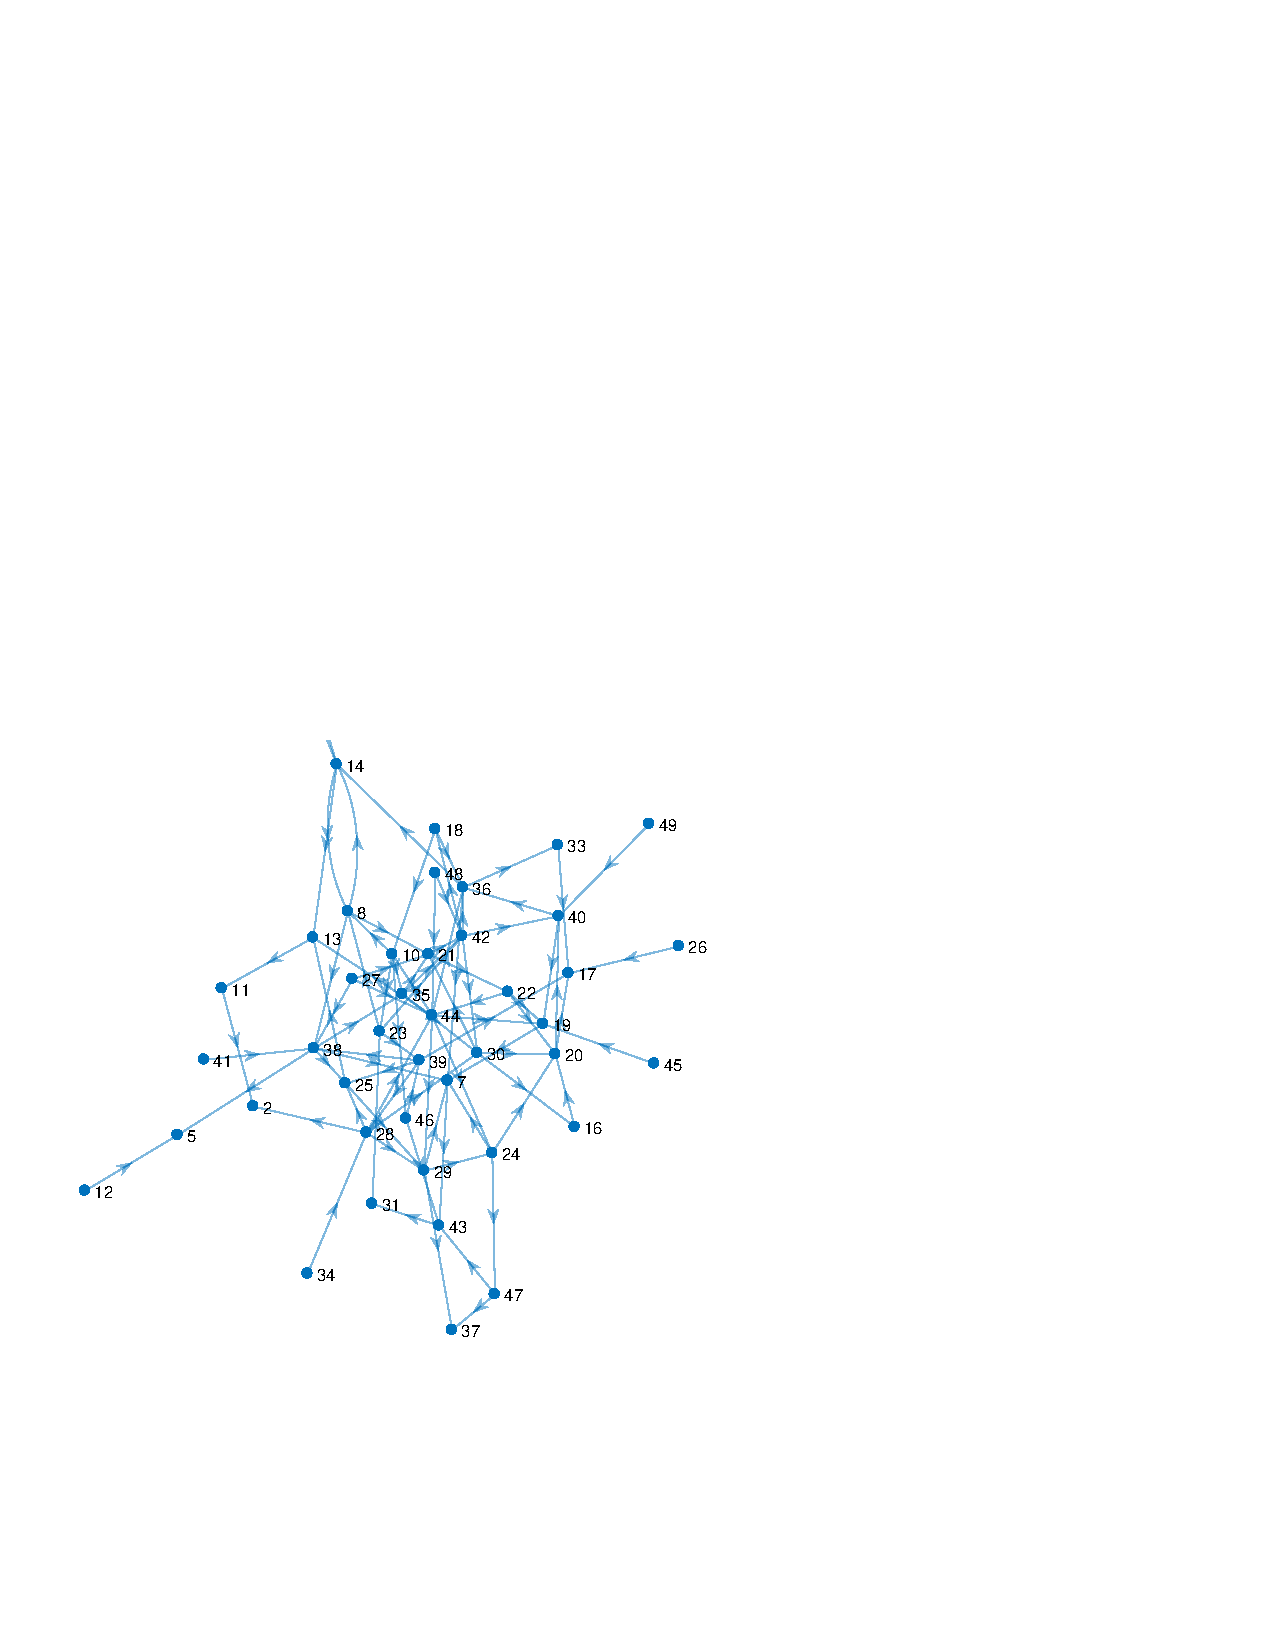
\includegraphics[width=0.8\linewidth]{dag}
%\caption{A Directed Acyclic Graph of the Running AUTOSAR Software Application, Runnables = 50, Paths = 35, Activation Patterns shown in Table \ref{tbl_requirements}.}
%\label{fig_application}
%\end{figure}
%\begin{center}
%\small
%\begin{minipage}{.5\textwidth}%
%\centering
%\begin{tabular}{@{}p{0.25cm}lll@{}}
%\toprule
%C& $r_i$ & $(e_{r_im_1}, e_{r_im_2}, e_{r_im_3})$ & $period$\\ \midrule
%\multirow{4}{4em}{c1} 
%&$r_1$ & (0.030, 0.060, 0.090) & 1\\
%&$r_2$ & (0.041, 0.081, 0.122) & 2\\
%&$r_3$ & (0.083, 0.167, 0.250)  & 5\\ 
%&$r_4$ & (0.310, 0.620, 0.930) & 10 \\[0.3em]
%\hline
%\multirow{2}{4em}{c2} 
%&$r_1$ & (0.310, 0.620, 0.930) & 10\\
%&$r_2$ & (0.310, 0.620, 0.930) & 10\\
%&$r_3$ & (0.310, 0.620, 0.930)  & 10\\ 
%&$r_4$ & (0.310, 0.620, 0.930) & 10 \\[0.3em]
%\hline
%\multirow{2}{4em}{c3} 
%&$r_1$ & (0.310, 0.620, 0.930) & 10\\
%&$r_2$ & (0.291, 0.583, 0.874)) & 10\\
%&$r_3$ & (0.291, 0.583, 0.874)  & 20\\ 
%&$r_4$ & (0.291, 0.583, 0.874) & 20 \\[0.3em]
%\hline
%\multirow{2}{4em}{c4} 
%&$r_1$ & (0.291, 0.583, 0.874) & 20\\
%&$r_2$ & (0.291, 0.583, 0.874)) & 10\\
%&$r_3$ & (0.291, 0.583, 0.874)  & 20\\ 
%&$r_4$ & (0.093, 0.186, 0.279) & 50 \\[0.3em]
%\hline
%\multirow{2}{4em}{c5} 
%&$r_1$ & (0.420, 0.841, 1.261) & 100\\
%&$r_2$ & (0.420, 0.841, 1.261)) & 100\\
%&$r_3$ & (0.420, 0.841, 1.261)  & 100\\ 
%&$r_4$ & (0.420, 0.841, 1.261) & 100 \\[0.3em]
%\bottomrule
%\end{tabular}
%\captionof{table}{Specification of Components.}
%\label{tbl_comps_config}
%\end{minipage}~
%\begin{minipage}{.45\textwidth}
%\begin{center}
%    \begin{tabular}{@{}lll@{}}
%    \toprule
%    Activation, $AP$ & Share & Time, ms \\ \midrule
%    $\tau_1$ & 50  & 50\\
%    $\tau_1\rightarrow\tau_2$ & 20  & 100\\
%    $\tau_1\rightarrow\tau_2\rightarrow\tau_3$ & 20  & 200\\
%    $\tau_1\rightarrow\tau_2\rightarrow\tau_3\rightarrow\tau_4$ & 10  & 400\\
%    \bottomrule
%    \end{tabular}
%    \captionof{table}{Activation Patters of Cause-effect Chains, their Share and End-to-end Timing Requirements.}
%    \label{tbl_requirements}
%\end{center}
%\begin{center}
%    \begin{tabular}{@{}llll@{}}
%    \toprule
%    M  & $P_{idle}$& $P_{busy}$& $\lambda$ \\ \midrule
%    $m_1$ & 50.0& 140.0 &1.0E-3  \\
%    $m_2$ & 10.0& 100.0 &1.0E-4  \\
%    $m_3$ & 10.0& 140.0 &1 .0E-5 \\ \bottomrule
%    \end{tabular}
%    \captionof{table}{Computation Nodes Specification.}
%    \label{tbl_nodes_specification}
%\end{center}
%\end{minipage}
%\end{center}

In the next section, we discuss our proposed method to address the considered optimization problem. 
